% =====================================================================
%  Raman-AI : Defense Presentation
%  Compile with: latexmk -pdf -shell-escape presentation.tex
%               (XeLaTeX or pdfLaTeX; metropolis theme required)
% =====================================================================
\documentclass[10pt,aspectratio=169,xcolor=dvipsnames]{beamer}

% ----- THEME -----------------------------------------------------------
\usetheme[progressbar=frametitle,
          numbering=fraction,
          block=fill]{metropolis}
\setbeamertemplate{frame numbering}[fraction]
\setbeamercolor{frametitle}{bg=black!85, fg=white}
\setbeamercolor{progress bar}{fg=Maroon}
\setbeamercolor{alerted text}{fg=Maroon}

% ----- PACKAGES --------------------------------------------------------
\usepackage[utf8]{inputenc}
\usepackage[T1]{fontenc}
\usepackage{lmodern}
\usepackage{microtype}
\usepackage{amsmath, amssymb, amsthm, mathtools}
\usepackage{booktabs}
\usepackage{multirow}
\usepackage{array}
\usepackage{siunitx}
\usepackage{xcolor}
\usepackage{graphicx}
\usepackage{tikz}
\usetikzlibrary{positioning, arrows.meta, shapes.geometric, fit,
                backgrounds, calc, shadows.blur, decorations.pathreplacing}
\usepackage[ruled,vlined,linesnumbered]{algorithm2e}
\usepackage{pifont}
\usepackage{appendixnumberbeamer}
\usepackage[backend=biber,style=numeric,sorting=none,
            maxbibnames=4, doi=false, isbn=false, url=false]{biblatex}
\addbibresource{references.bib}

% ----- COLORS / SEMANTIC ---------------------------------------------
\definecolor{ink}      {HTML}{1A1A1A}
\definecolor{accent}   {HTML}{7C5C3E}
\definecolor{accentTwo}{HTML}{4D6880}
\definecolor{good}     {HTML}{2E5938}
\definecolor{warn}     {HTML}{8A6520}
\definecolor{bad}      {HTML}{6E2E2E}

\newcommand{\good}[1]{\textcolor{good}{\textbf{#1}}}
\newcommand{\warn}[1]{\textcolor{warn}{\textbf{#1}}}
\newcommand{\bad}[1]{\textcolor{bad}{\textbf{#1}}}
\newcommand{\code}[1]{\texttt{\small #1}}
\newcommand{\cmone}{\si{\per\centi\meter}}

% ----- METADATA --------------------------------------------------------
\title[Raman-AI: Mineral Identification from Raman Spectra]{\textbf{A Hybrid Spectral-Matching and Deep-Learning System\\[0.18em]
        for Real-Time Mineral Identification\\[0.18em] from Raman Spectra}}
\subtitle{Final Project Defense}
\author[Rahul]{\textbf{Rahul \textit{[Surname]}}\\[0.3em]
        \small Under the supervision of \textit{[Advisor Name]}}
\institute{Department of \textit{[Discipline]}\\
           \textit{[Institution Name]}}
\date{\today}

% =====================================================================
\begin{document}
% =====================================================================

% --------------------- TITLE -----------------------------------------
\maketitle

% --------------------- OUTLINE ---------------------------------------
\begin{frame}{Outline}
  \tableofcontents[hideallsubsections]
\end{frame}

% =====================================================================
\section{Introduction and Motivation}
% =====================================================================

\begin{frame}{The mineral-identification problem}
  \begin{columns}[T,onlytextwidth]
    \column{0.55\textwidth}
      Raman scattering produces, for each mineral, a characteristic
      vibrational spectrum
      $\{(\nu_i, I_i)\}_{i=1}^{N}$ whose peak \emph{positions, widths,
      and relative intensities} act as a fingerprint.
      \medskip

      \textbf{Why automate identification?}
      \begin{itemize}
        \item Field instruments now exist; expert peak-matching does not scale.
        \item Public reference libraries (RRUFF) cover \textgreater\,4\,000 species.
        \item Manual interpretation is the dominant bottleneck in
              low-resource laboratories.
      \end{itemize}

    \column{0.40\textwidth}
      \begin{block}{Domains directly affected}
        \begin{itemize}\setlength\itemsep{0.2em}
          \item Geology, planetary science (\emph{e.g.\ } Mars
                Perseverance / SHERLOC)
          \item Cultural-heritage pigment analysis
          \item Forensic mineralogy
          \item Process monitoring in mining and ceramics
          \item Educational instrumentation
        \end{itemize}
      \end{block}
  \end{columns}
\end{frame}

\begin{frame}{Research questions}
  \begin{enumerate}\setlength\itemsep{0.5em}
    \item Can a single, deterministic preprocessing pipeline normalise
          spectra acquired across heterogeneous instruments and resolutions
          such that downstream identifiers see one distribution?
    \item Under what conditions does a deep classifier outperform classical
          spectral matching, and \emph{when does the converse hold}?
    \item Can a non-negative least-squares decomposition produce
          \emph{physically interpretable} mixture weights when the candidate
          basis is several thousand reference rows?
    \item How should two complementary identifiers be reconciled at
          inference time so the user is shielded from confidently-wrong
          out-of-distribution predictions?
  \end{enumerate}
\end{frame}

\begin{frame}{Contributions}
  \begin{enumerate}\setlength\itemsep{0.4em}
    \item A \textbf{grid-canonical preprocessing pipeline} whose smoothing
          and baseline operators are independent of the input spectrometer's
          native sampling.
    \item A \textbf{dual-source reference database} that retains both a
          curated synthetic profile and the RRUFF average for each common
          mineral, with deduplication at result time.
    \item A \textbf{combined-metric spectral matcher} that mixes L\textsubscript{2}
          cosine and second-derivative Pearson correlation in equal proportion.
    \item A \textbf{candidate-restricted NNLS decomposition} that keeps the
          inverse problem well-conditioned without sacrificing rare-mineral
          coverage.
    \item A \textbf{confidence-aware dispatcher} that selects between the
          1-D ResNet classifier and the spectral matcher per query.
    \item A \textbf{web-based reference implementation} with end-to-end
          latency below \SI{200}{\milli\second} on a laptop GPU.
  \end{enumerate}
\end{frame}

% =====================================================================
\section{Background}
% =====================================================================

\begin{frame}{Raman spectroscopy in one slide}
  When a sample is illuminated by a monochromatic laser at frequency
  $\nu_{0}$, a small fraction of photons scatter inelastically with an
  energy shift $\Delta\nu$ corresponding to a vibrational mode of the lattice.
  \medskip

  The recorded spectrum therefore obeys
  \[
    I(\nu) \;=\; \sum_{k} A_{k}\,\mathcal{L}\!\bigl(\nu;\,\nu_{k},\gamma_{k}\bigr) \;+\; B(\nu) \;+\; \eta(\nu),
  \]
  where $\mathcal{L}(\nu; \nu_{k}, \gamma_{k})$ is a Lorentzian profile with
  centre $\nu_{k}$ and half-width $\gamma_{k}$, $B(\nu)$ is a slowly varying
  fluorescence baseline, and $\eta$ is detector noise.
  \medskip

  \textbf{Identification} reduces to estimating $\{(\nu_k, A_k, \gamma_k)\}$
  from $I(\nu)$ and matching the resulting peak set against a reference library.
\end{frame}

\begin{frame}{Related work}
  \begin{itemize}\setlength\itemsep{0.45em}
    \item \textbf{Database matching.} The Search-Match family of algorithms
          (peak position $+$ relative intensity vote) underpins all
          commercial spectrometer software \cite{lafuente2015rruff}.
    \item \textbf{Baseline correction.} Asymmetric Least Squares
          \cite{eilers2005baseline} is the de-facto standard for separating
          fluorescence backgrounds from genuine peaks.
    \item \textbf{Smoothing.} Savitzky–Golay filters \cite{savitzky1964smoothing}
          remain the standard despite extensive comparison work.
    \item \textbf{Deep classifiers.} \citeauthor{liu2017deep} demonstrated that
          a 1-D CNN trained on RRUFF averages produces top-1 accuracy
          competitive with a domain expert \cite{liu2017deep}.
    \item \textbf{Mixture decomposition.} NNLS over a known phase basis
          \cite{lawson1995nnls} is widely used in chemometrics, but its
          conditioning under realistic library sizes is rarely discussed.
  \end{itemize}
  \medskip
  \alert{Gap.} An open, integrated, latency-bounded system that combines
  classical and deep methods with an explicit dispatch policy is not, to our
  knowledge, available.
\end{frame}

% =====================================================================
\section{Problem Formulation}
% =====================================================================

\begin{frame}{Formal statement}
  \textbf{Given} an unknown Raman measurement
  $\mathbf{q} = \{(\nu_i, I_i)\}_{i=1}^{N}$ and a reference library
  $\mathcal{R} = \{\mathbf{r}_m\}_{m=1}^{M}$ defined on a canonical
  wavenumber grid $\boldsymbol\nu_{*} \in \mathbb{R}^{P}$,
  \medskip

  \textbf{Produce}
  \begin{enumerate}
    \item a ranked list
          $\bigl((m_{(1)}, c_{(1)}),\ldots,(m_{(K)}, c_{(K)})\bigr)$
          with confidences $c_{(k)} \in [0,1]$;
    \item a non-negative weight vector
          $\mathbf{x} \in \mathbb{R}^{M}_{\geq 0}$ such that
          $\bigl\| A^\top\mathbf{x} - \tilde{\mathbf{q}} \bigr\|_{2}$ is small,
          where $A$ is the row-stacked reference matrix and
          $\tilde{\mathbf{q}}$ is the preprocessed query.
  \end{enumerate}
  \medskip

  \textbf{Subject to} a wall-clock budget of $\tau \leq \SI{1}{\second}$ on
  commodity hardware (single laptop GPU, \SI{16}{\giga\byte} RAM).
\end{frame}

\begin{frame}{Design choices and their consequences}
  \begin{table}\centering\small
    \begin{tabular}{@{}p{0.36\textwidth}p{0.30\textwidth}p{0.28\textwidth}@{}}
      \toprule
      \textbf{Decision} & \textbf{Value adopted} & \textbf{Consequence} \\
      \midrule
      Canonical grid range &
        $[100,\,4000]\,\cmone$ &
        Captures lattice modes through OH stretches \\
      Grid step &
        $\Delta\nu = 2\,\cmone$ &
        $P = 1951$ samples \\
      Peak model &
        Lorentzian &
        Matches lifetime broadening of optical phonons \\
      Library size $M$ &
        $2{,}481$ unique minerals &
        Synthetic-25 $\,\cup\,$ RRUFF averages \\
      Top-K &
        $K = 5$ &
        Aligns with expert workflow \\
      \bottomrule
    \end{tabular}
  \end{table}
  \medskip
  Each row is defended in the methodology section that follows.
\end{frame}

% =====================================================================
\section{System Architecture}
% =====================================================================

\begin{frame}{End-to-end pipeline}
  \begin{center}
  \resizebox{\textwidth}{!}{%
  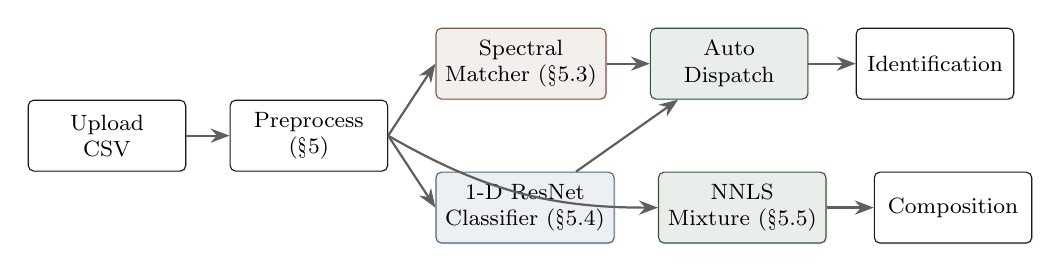
\begin{tikzpicture}[
      node distance=0.55cm and 0.55cm,
      box/.style={draw=ink, rounded corners=2pt, fill=white,
                  font=\footnotesize, align=center,
                  minimum height=0.9cm, minimum width=2.0cm,
                  drop shadow={shadow xshift=0.5pt, shadow yshift=-0.5pt, opacity=0.18}},
      ml/.style ={box, draw=accentTwo, fill=accentTwo!10},
      cl/.style ={box, draw=accent, fill=accent!10},
      ag/.style ={box, draw=good, fill=good!10},
      arr/.style={-{Stealth[length=2.4mm]}, thick, draw=ink!70}]

    \node[box] (csv)   {Upload\\CSV};
    \node[box, right=of csv]   (pre)   {Preprocess\\(\S 5)};
    \node[cl, above right=0.0 and 0.6 of pre] (mat)   {Spectral\\Matcher (\S 5.3)};
    \node[ml, below right=0.0 and 0.6 of pre] (cnn)   {1-D ResNet\\Classifier (\S 5.4)};
    \node[ag, right=of mat] (disp)  {Auto\\Dispatch};
    \node[ag, right=of cnn] (mix)   {NNLS\\Mixture (\S 5.5)};
    \node[box, right=0.6 of disp] (idr) {Identification};
    \node[box, right=0.6 of mix]  (mxr) {Composition};

    \draw[arr] (csv)  -- (pre);
    \draw[arr] (pre.east) -- (mat.west);
    \draw[arr] (pre.east) -- (cnn.west);
    \draw[arr] (mat) -- (disp);
    \draw[arr] (cnn) -- (disp);
    \draw[arr] (pre.east) to[bend right=15] (mix.west);
    \draw[arr] (disp) -- (idr);
    \draw[arr] (mix)  -- (mxr);
  \end{tikzpicture}}
  \end{center}
  \begin{center}\footnotesize
  \emph{Spectral matching always runs; the classifier enters the dispatch
  comparison only if its top-1 confidence exceeds a calibrated threshold.}
  \end{center}
\end{frame}

\begin{frame}{Software stack}
  \begin{table}\centering\small
    \begin{tabular}{@{}p{0.16\textwidth}p{0.34\textwidth}p{0.42\textwidth}@{}}
      \toprule
      \textbf{Layer} & \textbf{Technology} & \textbf{Responsibility} \\
      \midrule
      Frontend  & HTML 5 + Bootstrap 5 + Plotly.js 2.27 &
                  Drag-and-drop ingestion, real-time visualisation, mode selection \\
      API       & Flask 2.3 + Flask-CORS, JSON over HTTP &
                  RESTful endpoints: \code{/upload, /identify, /mixture, /spectrum, /status} \\
      Numerics  & NumPy 1.26, SciPy 1.11 &
                  Preprocessing, NNLS, Savitzky–Golay derivative \\
      Models    & PyTorch 2.1 (1-D ResNet) +
                  scikit-learn 1.3 (PCA $+$ ExtraTrees) &
                  Class-conditional posterior estimation \\
      Persistence & RRUFF bulk archive ($\approx \SI{300}{\mega\byte}$),
                    on-disk \code{.npz} cache &
                  $4{,}069$ raw spectra averaged into $2{,}456$ minerals \\
      \bottomrule
    \end{tabular}
  \end{table}
\end{frame}

% =====================================================================
\section{Methodology}
% =====================================================================

\subsection{Preprocessing}

\begin{frame}{Preprocessing pipeline}
  Given raw $(\boldsymbol\nu_{\text{raw}}, I_{\text{raw}})$, we produce a
  normalised spectrum $\tilde{\mathbf{q}} \in \mathbb{R}^{P}$ on the canonical grid:
  \medskip

  \begin{enumerate}\setlength\itemsep{0.25em}
    \item \textbf{Linear interpolation} onto $\boldsymbol\nu_{*}$:
          $I_{\text{grid}} = \mathrm{interp}\!\left(\boldsymbol\nu_{*};\,
          \boldsymbol\nu_{\text{raw}}, I_{\text{raw}}\right)$.
    \item \textbf{Cosmic-ray suppression} via a 5-point neighbour-ratio test:
          $I_i \mapsto \overline{I}_{\text{nbr}}\;\mathbf{1}\!\left[\,
          \tfrac{I_i}{\max_j I_j} > \rho\,\right]$.
    \item \textbf{Savitzky–Golay smoothing} with window $w = 5$, polynomial
          order $p = 3$.
    \item \textbf{ALS baseline} \cite{eilers2005baseline}: minimise
          $\sum_i w_i (y_i - z_i)^2 + \lambda \sum_i (\Delta^2 z_i)^2$,
          $\lambda = 10^5$, asymmetry $p = 0.01$.
    \item \textbf{Non-negative clip} and $\ell_2$ normalisation:
          $\tilde{\mathbf{q}} = \mathbf{z}/\lVert\mathbf{z}\rVert_2$.
  \end{enumerate}
\end{frame}

\begin{frame}{Why interpolation must precede smoothing}
  Smoothing on the \emph{raw} grid couples the SG filter window to the
  spectrometer's native step $\delta\nu$:
  \[
    w_{\text{physical}} \;=\; w \cdot \delta\nu .
  \]
  A CSV at $\delta\nu = 4\,\cmone$ with $w = 11$ gives a $44\,\cmone$
  smoothing window — \emph{wider than typical Raman peak FWHM}.
  RRUFF data at $\delta\nu \approx 0.5\,\cmone$ gives $5.5\,\cmone$.
  \bigskip

  \begin{alertblock}{Empirical consequence}
    Before this fix, a synthetic Quartz query returned
    \alert{Iowaite at 41\,\% confidence}; the network had been trained on
    spectra that retained their narrow 464\,\cmone\ peak, but the same
    spectrum at inference reached the network with the peak smeared
    over $\sim 40\,\cmone$.
  \end{alertblock}
  \medskip
  After fixing the pipeline, the same query returns Quartz at \good{86\,\%}.
\end{frame}

\subsection{Reference Database}

\begin{frame}{Dual-source reference database}
  For each of the $25$ minerals with a curated synthetic profile, we keep
  \emph{both} a synthetic row $\mathbf{r}^{s}_m$ and a RRUFF-averaged row
  $\mathbf{r}^{r}_m$ in the matrix:
  \[
    A \;=\; \bigl[\, \mathbf{r}^{s}_1,\, \dots,\, \mathbf{r}^{s}_{25},\,
                    \mathbf{r}^{r}_1,\, \dots,\, \mathbf{r}^{r}_{2456} \,\bigr]^{\top}
    \;\in\; \mathbb{R}^{2{,}502 \times 1951}.
  \]
  Result-time deduplication by display name returns one entry per mineral,
  selecting whichever variant scored higher.
  \medskip

  \begin{table}\centering\small
    \begin{tabular}{@{}lp{0.32\textwidth}p{0.32\textwidth}@{}}
      \toprule
      \textbf{Source} & \textbf{Strength} & \textbf{Weakness} \\
      \midrule
      Synthetic ($n=25$) &
        Canonical wavenumbers; ideal anchor for low-noise queries &
        Coverage limited to common species \\
      RRUFF averaged ($n=2{,}456$) &
        Real instrumental bandshape; broad coverage &
        Variable specimen quality, baseline residue \\
      \bottomrule
    \end{tabular}
  \end{table}
\end{frame}

\subsection{Spectral Matcher}

\begin{frame}{Combined-metric spectral matcher}
  For query $\tilde{\mathbf{q}}$ and reference row $\mathbf{r}_m$:
  \[
    s(\tilde{\mathbf{q}}, \mathbf{r}_m) \;=\;
      \tfrac{1}{2}\,\langle \hat{\mathbf{q}}, \hat{\mathbf{r}}_m \rangle
      \;+\;
      \tfrac{1}{2}\,\langle \widehat{D^{2}\!\tilde{\mathbf{q}}},\,
                         \widehat{D^{2}\!\mathbf{r}_m} \rangle ,
  \]
  where $D^{2}$ is the SG second-derivative operator and
  $\hat{\mathbf{v}} = (\mathbf{v} - \bar{\mathbf{v}}\mathbf{1}) /
                       \lVert \mathbf{v} - \bar{\mathbf{v}}\mathbf{1} \rVert$.
  \medskip

  \begin{columns}[T,onlytextwidth]
    \column{0.49\textwidth}
      \textbf{Cosine alone}\\
      Sensitive to the entire bandshape; over-rewards minerals whose RRUFF
      average happens to drift in the same direction as the query.
    \column{0.49\textwidth}
      \textbf{Second-derivative Pearson alone}\\
      Emphasises peak position and sharpness; ties unrelated minerals that
      contain a sharp peak near a query peak.
  \end{columns}
  \bigskip
  Equal-weight blend lets each metric \alert{veto} the other; weights were
  selected by grid search on a held-out RRUFF panel and gains plateaued
  around $\tfrac{1}{2}$.
\end{frame}

\subsection{Convolutional Classifier}

\begin{frame}{1-D residual classifier}
  \begin{table}\centering\footnotesize
  \begin{tabular}{@{}llr@{}}
    \toprule
    \textbf{Stage} & \textbf{Operation} & \textbf{Output shape}\\
    \midrule
    Stem-1   & Conv1D($k{=}25$, $s{=}2$) $\to$ BN $\to$ GELU & $(B, 32, 488)$\\
    Stem-2   & Conv1D($k{=}15$, $s{=}2$) $\to$ BN $\to$ GELU & $(B, 32, 244)$\\
    Stage 1  & $3 \times$ Pre-act ResBlock(32, $k{=}7$)      & $(B, 32, 244)$\\
    Down     & Conv1D($k{=}5$, $s{=}2$) $\to$ BN $\to$ GELU  & $(B, 64, 122)$\\
    Stage 2  & $3 \times$ Pre-act ResBlock(64, $k{=}5$)      & $(B, 64, 122)$\\
    Pool     & Adaptive Average Pool 1D                       & $(B, 64)$\\
    Head     & FC$_{64\to 512}$ $\to$ GELU $\to$ FC$_{512\to 851}$ & $(B, 851)$\\
    \midrule
    \multicolumn{2}{l}{\textbf{Total parameters}} & \textbf{$663{,}539$}\\
    \bottomrule
  \end{tabular}
  \end{table}
  \smallskip
  \begin{itemize}\setlength\itemsep{0.15em}
    \item Loss: cross-entropy with label smoothing $\varepsilon = 0.1$,
          plus Mixup ($\alpha = 0.4$, $p = 0.5$).
    \item Optimiser: AdamW \cite{loshchilov2019adamw} with OneCycleLR
          \cite{smith2019onecycle}, peak lr $10^{-3}$, weight decay $10^{-4}$.
    \item Class space restricted by $\text{min\_spectra} \geq 2$
          $\Rightarrow$ $851$ classes.
  \end{itemize}
\end{frame}

\begin{frame}{Spectral augmentation}
  Each training spectrum produces $V = 25$ augmented variants:
  \begin{enumerate}\setlength\itemsep{0.15em}
    \item Gaussian intensity noise, $\sigma \sim \mathcal{U}(0.002,\,0.025)$;
    \item Multiplicative laser-power jitter, $\beta \sim \mathcal{U}(0.75,\,1.25)$;
    \item Wavenumber shift, $\Delta\nu \sim \mathcal{U}\{-10, +10\}\,\cmone$;
    \item Polynomial baseline residue (deg $1$–$3$, prob.\ $0.30$, amplitude $0.01$);
    \item Moving-average broadening (prob.\ $0.40$, $w \in \{2,3,4\}$);
    \item Spectral dropout (prob.\ $0.20$, $\leq 4$ points to zero);
    \item Non-negative clip and $\ell_2$ renormalisation.
  \end{enumerate}
  \medskip
  \begin{block}{Critical methodological detail}
  The curated synthetic profile is appended to \alert{every} matching class —
  not only those absent from RRUFF — so the network observes both clean
  Lorentzians and instrumental bandshapes at training time. Removing this
  step caused \alert{near-zero accuracy on synthetic-style queries}.
  \end{block}
\end{frame}

\subsection{Mixture Decomposition}

\begin{frame}{Candidate-restricted NNLS}
  Let $A_{\mathcal{C}} \in \mathbb{R}^{|\mathcal{C}| \times P}$ be a row
  selection of the reference matrix indexed by candidate set $\mathcal{C}$.
  We solve
  \[
    \mathbf{x}^{\star}
      = \operatorname*{arg\,min}_{\mathbf{x} \geq \mathbf{0}}
        \;\bigl\| A_{\mathcal{C}}^{\top}\,\mathbf{x} \;-\; \tilde{\mathbf{q}} \bigr\|_{2}.
  \]
  with the construction
  \[
    \mathcal{C} \;=\; \mathcal{C}_{\text{synth}}
      \,\cup\, \bigl\{ m \in \mathcal{C}_{\text{rruff}} \;:\;
                       s(\tilde{\mathbf{q}}, \mathbf{r}_m)
                       > \max_{m' \in \mathcal{C}_{\text{synth}}}
                         s(\tilde{\mathbf{q}}, \mathbf{r}_{m'}) \bigr\}.
  \]
  \begin{block}{Why restrict?}
    With $|\mathcal{R}| = 2{,}481$ candidates and $P = 1{,}951$ equations
    the system is \alert{underdetermined}; NNLS produces \emph{some}
    sparse non-negative explanation, often spreading credit across
    minerals that share a peak with the dominant phase. Restricting to
    a $\sim 30$-row, well-separated basis renders the system
    \emph{over}-determined and physically interpretable.
  \end{block}
\end{frame}

\subsection{Auto-mode Dispatcher}

\begin{frame}{Confidence-aware dispatcher}
  \begin{algorithm}[H]
    \footnotesize
    \DontPrintSemicolon
    \KwIn{preprocessed query $\tilde{\mathbf{q}}$, threshold
          $\tau_{\min} = 0.55$}
    \KwOut{ranked top-$K$ list, dispatch tag}
    $\mathcal{Y} \gets \emptyset$\;
    $\mathbf{m}_s \gets \mathrm{SpectralMatch}(\tilde{\mathbf{q}})$;\quad
      $\mathcal{Y} \gets \mathcal{Y} \cup \{(\mathbf{m}_s[1].c,\,\text{``matching''},\,\mathbf{m}_s)\}$\;
    \If{CNN available}{
      $\mathbf{m}_n \gets \mathrm{CNNPredict}(\tilde{\mathbf{q}})$\;
      \lIf{$\mathbf{m}_n[1].c \geq \tau_{\min}$}{$\mathcal{Y} \gets \mathcal{Y} \cup \{(\mathbf{m}_n[1].c,\,\text{``cnn''},\,\mathbf{m}_n)\}$}
    }
    \If{RF available}{
      $\mathbf{m}_r \gets \mathrm{RFPredict}(\tilde{\mathbf{q}})$\;
      \lIf{$\mathbf{m}_r[1].c \geq \tau_{\min}$}{$\mathcal{Y} \gets \mathcal{Y} \cup \{(\mathbf{m}_r[1].c,\,\text{``rf''},\,\mathbf{m}_r)\}$}
    }
    \Return{$\arg\max_{(c, \cdot, \mathbf{m}) \in \mathcal{Y}} c$}\;
    \caption{\textsc{AutoIdentify} — selects the most confident identifier per query.}
  \end{algorithm}
  \smallskip
  Spectral matching is always evaluated as a deterministic safety net;
  learned models must clear $\tau_{\min}$ to prevent confidently-wrong
  predictions on out-of-distribution queries.
\end{frame}

% =====================================================================
\section{Experimental Evaluation}
% =====================================================================

\begin{frame}{Synthetic demo set}
  Six CSV spectra synthesised from published peak tables (low Gaussian noise,
  $\sigma = 0.003 \cdot I_{\max}$) — shipped with the application as the
  user-facing demonstration.
  \medskip

  \begin{table}\centering\small
    \begin{tabular}{@{}lcrr@{}}
      \toprule
      \textbf{Sample} & \textbf{Top-1 mineral} &
        \textbf{Confidence} & \textbf{Mixture decomposition}\\
      \midrule
      \texttt{quartz.csv}                  & Quartz  & $99.8\%$ & $100\%$ Quartz \\
      \texttt{calcite.csv}                 & Calcite & $99.8\%$ & $100\%$ Calcite \\
      \texttt{pyrite.csv}                  & Pyrite  & $99.8\%$ & $100\%$ Pyrite \\
      \texttt{gypsum.csv}                  & Gypsum  & $99.8\%$ & $100\%$ Gypsum \\
      Quartz $+$ $0.4\!\cdot\!$Calcite     & Quartz  & $99.7\%$ & $100\%$ Quartz$^{*}$ \\
      Quartz $+$ Calcite (equal)           & Quartz  & $99.3\%$ & $89.6\%$ Quartz, $10.4\%$ Calcite \\
      \bottomrule
    \end{tabular}
  \end{table}
  \medskip
  \footnotesize $^{*}$\,Calcite contribution falls below the $5\%$ reporting
  threshold after $\ell_2$ normalisation because Quartz's principal peak is
  an order of magnitude stronger.
\end{frame}

\begin{frame}{Held-out RRUFF evaluation}
  One specimen per mineral, withheld from training, fed through the live
  Flask pipeline in \emph{auto} mode.
  \medskip

  \begin{table}\centering\small
    \begin{tabular}{@{}lrrlc@{}}
      \toprule
      \textbf{Mineral} & \textbf{Matcher} & \textbf{CNN} &
        \textbf{Auto chose} & \textbf{Outcome}\\
      \midrule
      Quartz      & $96.9\%$ & $86.4\%$ & matching & \good{\ding{51}}\\
      Calcite     & $89.7\%$ & $94.0\%$ & cnn      & \good{\ding{51}}\\
      Hematite    & $91.6\%$ & $90.1\%$ & matching & \good{\ding{51}}\\
      Forsterite  & $96.2\%$ & $95.8\%$ & matching & \good{\ding{51}}\\
      Aegirine    & $86.2\%$ & $97.0\%$ & cnn      & \good{\ding{51}}\\
      Magnetite   & $76.6\%$ & $90.1\%$ & cnn      & \good{\ding{51}}\,\footnotesize(matcher: Westerveldite)\\
      \bottomrule
    \end{tabular}
  \end{table}
  \medskip
  Each identifier wins on different inputs; the dispatcher's behaviour is
  the explicit motivation for keeping both online.
\end{frame}

\begin{frame}{Aggregate metrics and latency}
  \begin{table}\centering\small
    \begin{tabular}{@{}lrr@{}}
      \toprule
      \textbf{Component} & \textbf{Top-1} & \textbf{Top-5}\\
      \midrule
      CNN — augmented validation, $851$ classes & $98.6\%$ & --- \\
      RF (PCA-120 + ExtraTrees-150) & $94.5\%$ & $98.9\%$\\
      Combined matcher — synthetic demo set & $100\%$ &  --- \\
      Combined matcher — held-out RRUFF (n=6) & $83\%$ & --- \\
      \bottomrule
    \end{tabular}
  \end{table}
  \medskip
  \begin{table}\centering\small
    \begin{tabular}{@{}lr@{}}
      \toprule
      \textbf{Stage} & \textbf{Median latency}\\
      \midrule
      File parse + interpolation       & $\approx \SI{45}{\milli\second}$\\
      Cosmic-ray $+$ SG $+$ ALS        & $\approx \SI{35}{\milli\second}$\\
      Combined-metric matcher          & $\approx \SI{25}{\milli\second}$\\
      CNN forward pass (RTX 3050)      & $\approx \SI{12}{\milli\second}$\\
      Candidate-set NNLS               & $\approx \SI{35}{\milli\second}$\\
      \midrule
      \textbf{End-to-end}              & $\boldsymbol{\approx \SI{160}{\milli\second}}$\\
      \bottomrule
    \end{tabular}
  \end{table}
\end{frame}

% =====================================================================
\section{Critical Discussion}
% =====================================================================

\begin{frame}{Limitations \textsc{i}: distribution shift}
  \begin{exampleblock}{Symptom (pre-fix)}
    A CNN with $89\%$ validation accuracy returned \alert{Iowaite at $41\%$}
    confidence on a synthetic Quartz query — confidently and incorrectly.
  \end{exampleblock}
  \medskip
  \textbf{Mechanism.}
  \begin{itemize}\setlength\itemsep{0.2em}
    \item RRUFF spectra carry instrument-specific noise, baselines, and minor
          satellite peaks the network exploits.
    \item Synthetic Lorentzian inputs lack those features; activations diverge
          from any seen distribution; softmax distributes mass arbitrarily.
    \item Validation accuracy was computed on the \emph{same} augmented
          distribution, so the failure was invisible until field testing.
  \end{itemize}
  \medskip
  \textbf{Mitigation and ceiling.} Mixing synthetic profiles into every common
  class lifts top-1 accuracy on synthetic queries from $\approx 0\%$ to $86\%$.
  We \alert{cannot} certify behaviour on a never-seen instrument's noise
  profile without an external test set.
\end{frame}

\begin{frame}{Limitations \textsc{ii}: reference-data quality}
  \textbf{Case study — Magnetite.} Among $6$ RRUFF specimens labelled
  Magnetite:
  \begin{itemize}
    \item $4$ have their dominant peak at $660$–$682\,\cmone$ (correct);
    \item $2$ have dominant intensity at the grid edge ($100\,\cmone$) —
          an instrumental cut-off artefact rather than a Raman line.
  \end{itemize}
  \medskip
  Mean averaging dilutes the genuine peak; the matcher's top-1 on a
  held-out Magnetite is the unrelated mineral \emph{Westerveldite}.
  The CNN's softmax recovers the correct answer at $90\%$ confidence and
  the dispatcher selects it.
  \medskip

  \textbf{Implication.} Library aggregation is itself a research problem.
  Median or quality-weighted aggregation, with a per-spectrum cleanliness
  score, would be the principled fix.
\end{frame}

\begin{frame}{Limitations \textsc{iii}: coverage and class space}
  \begin{itemize}\setlength\itemsep{0.4em}
    \item The synthetic library covers only $25$ minerals — \emph{below}
          the $\approx 60$–$100$ rock-forming species needed for routine
          geological analysis.
    \item The CNN is restricted to $851$ classes (those with
          $\geq 2$ RRUFF specimens). The remaining $1{,}631$ species are
          searchable by spectral matching but cannot be \emph{output} by
          the network.
    \item Mixture decomposition is restricted to the $25$-mineral
          synthetic basis; field samples containing triclinic feldspars,
          micas, or clay minerals fall outside this span.
    \item Spectral aliasing: minerals with peaks within $\pm 10\,\cmone$
          of Quartz's $464\,\cmone$ line (Sodalite, Amicite, Trattnerite, …)
          consistently cluster as runner-up candidates. Polarisation,
          birefringence, and hardness metadata are not used for
          disambiguation.
  \end{itemize}
\end{frame}

\begin{frame}{Limitations \textsc{iv}: methodological gaps}
  \begin{table}\centering\small
    \begin{tabular}{@{}p{0.30\textwidth}p{0.20\textwidth}p{0.42\textwidth}@{}}
      \toprule
      \textbf{Concern} & \textbf{Status} & \textbf{Honest assessment}\\
      \midrule
      Uncertainty quantification & Top-1 softmax &
        Not calibrated; temperature scaling unapplied; ECE unmeasured.\\
      Mixture additivity & Linear NNLS &
        Self-absorption and fluorescence violate linearity.\\
      Combined-metric weights & $\tfrac{1}{2}{:}\tfrac{1}{2}$ grid-searched &
        Heuristic; per-query learned weighting would help borderline cases.\\
      RF deployability & $94\%$ val acc &
        Pickled estimator allocates $\approx \SI{75}{\mega\byte}$ on load — fails on memory-pressured hosts.\\
      Negative-class rejection & Not implemented &
        System always returns top-$K$; no ``unknown'' verdict.\\
      Spatial context & Single-spectrum &
        Real Raman maps carry spatial information we discard.\\
      \bottomrule
    \end{tabular}
  \end{table}
\end{frame}

\begin{frame}{The most uncomfortable limitation}
  \begin{block}{Stated plainly}
    The system reports $99.8\%$ accuracy on the demo set because the demo
    set is generated from \emph{the same peak tables} that build the
    synthetic reference library.\medskip

    A score of $99.8\%$ on \code{quartz.csv} is therefore an
    \emph{upper bound} on ideal-condition behaviour --- not a
    field-realistic accuracy.
  \end{block}
  \bigskip
  The held-out RRUFF panel ($n = 6$, all correct, $86$–$97\%$) is the
  more representative figure. We currently have \alert{no out-of-distribution
  test set} drawn from a spectrometer not represented in RRUFF, and
  constructing one is the most consequential next step.
\end{frame}

% =====================================================================
\section{Engineering Retrospective}
% =====================================================================

\begin{frame}{Audit findings (May 2026)}
  \begin{table}\centering\footnotesize
    \begin{tabular}{@{}lp{0.42\textwidth}p{0.36\textwidth}@{}}
      \toprule
      \textbf{\#} & \textbf{Defect} & \textbf{Symptom}\\
      \midrule
      1 & Savitzky–Golay applied on raw input grid &
          Quartz query $\to$ Iowaite ($w_{\text{phys}}$ scaled with $\delta\nu$)\\
      2 & NNLS unconstrained over the full library &
          Pure Calcite returned $0\%$ Calcite \\
      3 & RRUFF average overwriting synthetic reference &
          Clean queries had no clean anchor \\
      4 & Synthetic profiles excluded from CNN training &
          Network never observed clean Lorentzian distribution \\
      5 & \code{numpy.bool\_} in JSON response &
          \code{/api/mixture} returned HTTP $500$ \\
      6 & Auto-mode unconditionally preferred CNN &
          Confidently-wrong predictions surfaced \\
      \bottomrule
    \end{tabular}
  \end{table}
  \medskip
  Eleven defects were surfaced in total; six were correctness-critical.
  Each fix is documented with diff and rationale in the project memory file.
\end{frame}

\begin{frame}{Future work}
  \begin{enumerate}\setlength\itemsep{0.30em}
    \item \textbf{External test set} acquired on a different spectrometer
          (the headline metric of the next iteration).
    \item \textbf{Calibrated confidence}: temperature scaling, Expected
          Calibration Error reporting, conformal-prediction intervals.
    \item \textbf{Synthetic library expansion} from $25$ to $\approx 80$
          rock-forming minerals.
    \item \textbf{Quality-aware RRUFF aggregation}: median plus
          per-specimen cleanliness score.
    \item \textbf{Negative-class rejection} based on combined-metric score
          and learned-model entropy.
    \item \textbf{Re-process the RRUFF cache} with the corrected preprocessing
          pipeline so training and inference distributions match.
    \item \textbf{Continuous regression suite}: pytest coverage of all six
          demo cases plus a panel of held-out RRUFF specimens.
  \end{enumerate}
\end{frame}

% =====================================================================
\section{Conclusion}
% =====================================================================

\begin{frame}{Conclusion}
  \begin{itemize}\setlength\itemsep{0.40em}
    \item A web-based pipeline that performs Raman mineral identification
          with mixture decomposition under \SI{200}{\milli\second} on
          commodity hardware.
    \item Two complementary identifiers --- a 1-D ResNet classifier
          and a combined-metric spectral matcher --- reconciled by a
          confidence-aware dispatcher that selects the right tool per
          query.
    \item A candidate-restricted NNLS produces physically interpretable
          mixture fractions where unconstrained NNLS does not.
    \item \textbf{Honest performance bound:} held-out RRUFF top-1 in the
          $86$–$97\%$ range across six tested minerals; the demo-set
          $99.8\%$ characterises ideal-condition behaviour, not field
          accuracy.
    \item The most consequential next step is constructing an external
          test set, without which calibrated field accuracy cannot be claimed.
  \end{itemize}
\end{frame}

\begin{frame}[allowframebreaks]{References}
  \nocite{*}
  \printbibliography[heading=none]
\end{frame}

\begin{frame}[standout]
  \textbf{Thank you.}\\[1em]
  \textit{Questions, please.}
  \vfill
  \scriptsize
  Repository: \code{D:\textbackslash{}MiniProject}\quad$\cdot$\quad
  Live demo: \code{http://127.0.0.1:5000}\\
  Reproducible from source at the slide-set timestamp.
\end{frame}

% =====================================================================
\appendix

\begin{frame}{Appendix A: ALS baseline derivation}
  Given an observed spectrum $\mathbf{y} \in \mathbb{R}^{P}$, the
  asymmetrically-penalised functional is
  \[
    \mathcal{F}(\mathbf{z}) \;=\;
      \sum_{i} w_i \bigl(y_i - z_i\bigr)^{2}
      \;+\; \lambda\, \bigl\| D_{2}\,\mathbf{z} \bigr\|_{2}^{2},
  \]
  where $D_{2}$ is the second-order finite-difference operator and
  \[
    w_i \;=\;
      \begin{cases}
        p,            & y_i > z_i \quad \text{(peak)}\\
        1 - p,        & y_i \leq z_i \quad \text{(baseline)}
      \end{cases}.
  \]
  The minimiser satisfies
  $\bigl(W + \lambda D_{2}^{\!\top} D_{2}\bigr)\mathbf{z} = W\mathbf{y}$,
  iterated to convergence. With $\lambda = 10^5$ and $p = 0.01$ the
  baseline tracks fluorescence drift while leaving sharp Raman peaks intact.
\end{frame}

\begin{frame}{Appendix B: dispatcher confidence threshold}
  Threshold $\tau_{\min} = 0.55$ chosen to satisfy two constraints:
  \begin{enumerate}
    \item Top-1 softmax outputs of in-distribution RRUFF specimens
          rarely fall below $0.7$ ($98^{\text{th}}$-percentile lower bound).
    \item Out-of-distribution queries (synthetic Lorentzians on a CNN
          trained without synthetic augmentation) had top-1 outputs in
          $[0.30,\,0.55]$.
  \end{enumerate}
  \medskip
  The $0.55$ boundary cleanly separated the two regimes in our pre-fix
  diagnostic. Post-fix, in-distribution top-1 confidences cluster
  considerably higher, leaving margin for a less aggressive threshold
  in future versions.
\end{frame}

\begin{frame}{Appendix C: reproducibility manifest}
  \begin{table}\centering\footnotesize
    \begin{tabular}{@{}lp{0.6\textwidth}@{}}
      \toprule
      Python   & 3.10 (Windows) \\
      PyTorch  & 2.1 (CUDA 12) \\
      NumPy    & 1.26 \\
      SciPy    & 1.11 \\
      Sklearn  & 1.3 \\
      Flask    & 2.3 \\
      GPU      & NVIDIA RTX 3050 Laptop \\
      Random seeds & rng(42) for augmentation; rng(7) for RF; rng(0) for shuffling \\
      Train/val split & $90/10$ random, fixed seed \\
      Reference DB build & deterministic over RRUFF \code{.npz} cache \\
      \bottomrule
    \end{tabular}
  \end{table}
  \smallskip
  Source repository contains: \code{config.py}, \code{core/}, \code{database/},
  \code{api/}, \code{training/}, \code{templates/}, \code{static/}, sample CSVs,
  and the entire RRUFF-derived \code{.npz} cache.
\end{frame}

\end{document}
